% Manuel d'utilisation de Kab-board pour Word.
% Compilation : pdflatex manuel.tex, deux fois (sommaire et nombre de pages).

\documentclass[11pt,a4paper]{article}

\usepackage[a4paper,top=20mm,bottom=24mm,left=20mm,right=20mm,footskip=12mm]{geometry}
\usepackage{tipa}
\usepackage[T1]{fontenc}
\usepackage[utf8]{inputenc}
\usepackage{lmodern}
\usepackage{tgheros}
\renewcommand{\familydefault}{\sfdefault}
\usepackage{newunicodechar}
% Les lettres kabyles du texte.
\newunicodechar{ɣ}{\textipa{G}}
\newunicodechar{ḍ}{\d{d}}
\usepackage[french]{babel}
\frenchsetup{og=«, fg=», StandardItemLabels=true}
\usepackage{microtype}
\usepackage{xcolor}
\usepackage{graphicx}
\usepackage{tabularx,booktabs,array}
\usepackage{enumitem}
\usepackage{titlesec}
\usepackage{fancyhdr}
\usepackage{lastpage}
\usepackage{amssymb}
\usepackage[most]{tcolorbox}
\usepackage[hidelinks]{hyperref}
\hypersetup{pdftitle={Kab-board pour Word : manuel d'utilisation},pdfauthor={kab-board},pdflang={fr}}

\definecolor{vert}{HTML}{00843F}
\definecolor{bleu}{HTML}{0072BB}
\definecolor{ocre}{HTML}{A86A00}
\definecolor{encre}{HTML}{1F2328}
\definecolor{doux}{HTML}{59636E}
\definecolor{filet}{HTML}{D8DEE4}
\definecolor{fond}{HTML}{F6F8FA}
\color{encre}

\setlength{\parindent}{0pt}
\setlength{\parskip}{0.55em}
\linespread{1.08}
\setlist{itemsep=0.25em,topsep=0.3em,leftmargin=1.6em}

% Titres : un numéro vert, un filet sous le titre de section.
\titleformat{\section}{\Large\bfseries}{\textcolor{vert}{\thesection}\hspace{0.6em}}{0pt}{}[\vspace{0.25em}{\color{vert}\titlerule[1.2pt]}]
\titlespacing*{\section}{0pt}{1.6em}{0.9em}
\titleformat{\subsection}{\large\bfseries}{}{0pt}{}
\titlespacing*{\subsection}{0pt}{1.1em}{0.4em}

\pagestyle{fancy}
\fancyhf{}
\renewcommand{\headrulewidth}{0pt}
\fancyfoot[C]{\footnotesize\color{doux}Kab-board pour Word 0.3 \quad·\quad page \thepage\ sur \pageref*{LastPage}}

% Un bouton de Word ou du volet.
\newtcbox{\bouton}{on line, colback=fond, colframe=black!28, boxrule=0.4pt, arc=2pt,
  left=2.5pt, right=2.5pt, top=0.6pt, bottom=0.6pt, fontupper=\small}
% Un mot kabyle cité.
\newcommand{\kab}[1]{\textit{#1}}
% Un chemin de Windows.
\newcommand{\chemin}[1]{\texttt{#1}}
\newcommand{\bs}{\textbackslash}
\newcommand{\menu}{\enspace›\enspace}

% Encadrés.
\newtcolorbox{encadre}[2][bleu]{enhanced, breakable=false, colback=#1!7, colframe=#1,
  boxrule=0pt, leftrule=3.5pt, arc=0pt, outer arc=0pt, left=8pt, right=8pt, top=6pt, bottom=6pt,
  before skip=0.8em, after skip=0.9em, fontupper=\normalsize,
  before upper={\textbf{#2}\par\vspace{0.2em}}}

% Une capture, encadrée d'un filet, avec sa légende.
\newcommand{\capture}[3][\linewidth]{%
  \par\begin{center}
  \begin{tcolorbox}[enhanced, width=#1, boxrule=0.4pt, colframe=filet, colback=white, arc=3pt,
    left=0pt, right=0pt, top=0pt, bottom=0pt, boxsep=0pt]
  \includegraphics[width=\linewidth]{images/#2}
  \end{tcolorbox}\vspace{0.2em}
  {\small\color{doux}#3}
  \end{center}\par}

\newcolumntype{L}{>{\raggedright\arraybackslash}X}
\newcommand{\tableau}[3]{%
  \par\noindent\begin{tabularx}{\linewidth}{@{}>{\raggedright\arraybackslash}p{#1}L@{}}
  \toprule #2 \\ \midrule #3 \bottomrule
  \end{tabularx}\par}

\begin{document}

% ---------------------------------------------------------------- Couverture
\begin{titlepage}
\thispagestyle{empty}
\centering
\vspace*{18mm}
{\large\bfseries\color{vert}K\,A\,B\,-\,B\,O\,A\,R\,D\par}
\vspace{8mm}
{\fontsize{30}{36}\selectfont\bfseries Le correcteur kabyle\\[2mm] pour Microsoft Word\par}
\vspace{6mm}
{\Large\color{doux}Manuel d'utilisation · version 0.3\par}
\vspace{14mm}
\begin{tcolorbox}[enhanced, width=0.9\linewidth, boxrule=0.4pt, colframe=filet, colback=white, arc=4pt,
  left=0pt, right=0pt, top=0pt, bottom=0pt, boxsep=0pt, drop fuzzy shadow=black!35]
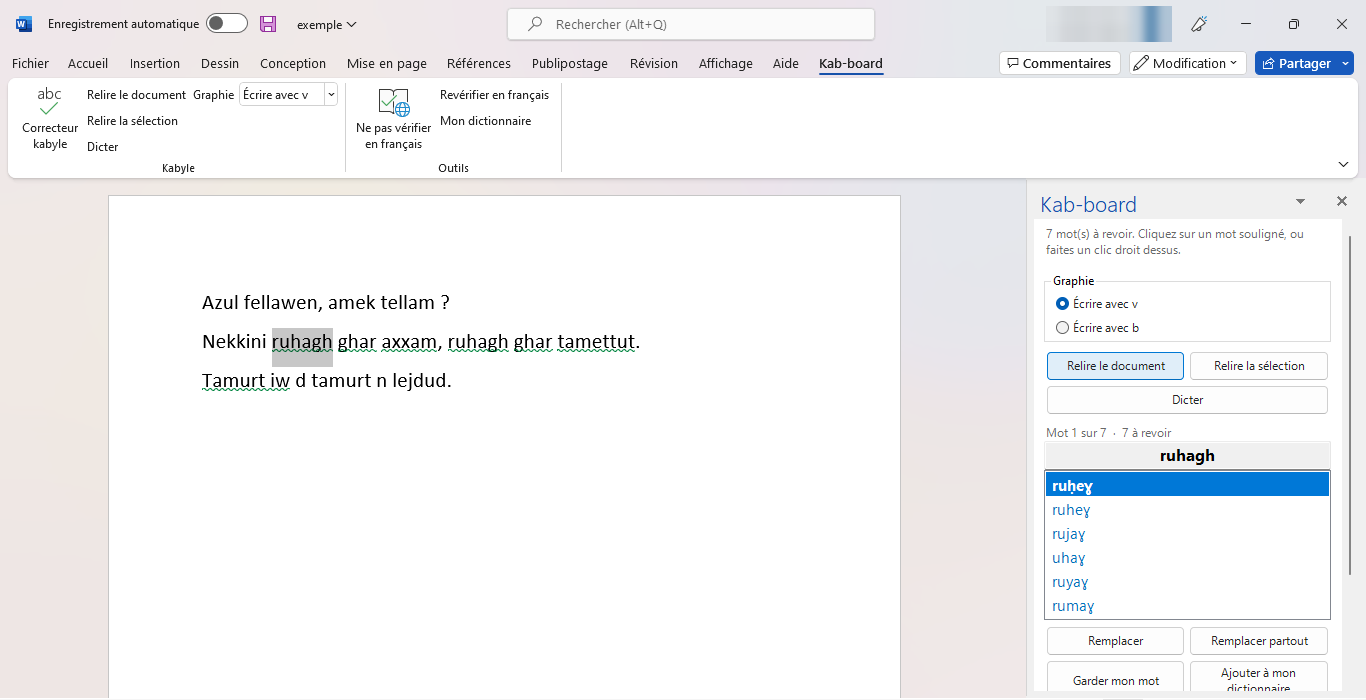
\includegraphics[width=\linewidth]{images/relecture.png}
\end{tcolorbox}
\vspace{14mm}
{\color{doux}Installation, relecture, corrections, dictée, désinstallation.\\
Tout se calcule sur votre ordinateur : rien n'est envoyé sur Internet.\par}
\vfill
{\footnotesize\color{doux}Kab-board, correcteur kabyle. Licence GNU GPL version 3 ou ultérieure.
Le modèle de langue et le lexique sont publiés sous licence CC BY-SA 4.0, doi 10.5281/zenodo.22112059.
La dictée utilise le modèle vocal Mmeslay (Aomer Gaya Ouldali), sous licence GNU GPL version 3.\par}
\end{titlepage}

% ---------------------------------------------------------------- Sommaire
\renewcommand{\contentsname}{Sommaire}
\setcounter{tocdepth}{1}
\tableofcontents
\newpage

% ---------------------------------------------------------------- 1
\section{Ce qu'il faut}\label{s:faut}
\begin{itemize}
  \item \textbf{Windows 10 ou 11}, en 64 bits (presque tous les ordinateurs récents).
  \item \textbf{Microsoft Word 2013 ou plus récent}, y compris Word de Microsoft 365.
  \item Environ \textbf{700 Mo} d'espace libre.
  \item Pour la dictée seulement : un \textbf{micro} (celui d'un portable, d'un casque ou d'une webcam suffit).
\end{itemize}
Il n'y a rien d'autre à installer. Le correcteur emporte tout avec lui : le lexique kabyle de 1,58 million de formes, le modèle de langue, le modèle de dictée, et le programme qui les fait tourner.

\begin{encadre}[ocre]{Ce qui ne marche pas}
Word pour Mac, Word en ligne (dans le navigateur) et Word sur téléphone n'acceptent pas ce genre de complément.
\end{encadre}

Pas besoin d'être administrateur de l'ordinateur : Kab-board s'installe dans votre compte Windows, comme une application personnelle.

% ---------------------------------------------------------------- 2
\section{Installer Kab-board}\label{s:installer}
L'installeur est un seul fichier : \chemin{kab-board-word-setup-0.3.exe} (environ 250 Mo).

\subsection{Étape 1 : lancer l'installeur}
Double-cliquez sur le fichier.
\begin{encadre}[ocre]{« Windows a protégé votre ordinateur »}
L'installeur n'est pas signé numériquement, alors Windows peut afficher cet écran bleu la première fois. Cliquez sur \bouton{Informations complémentaires}, puis sur \bouton{Exécuter quand même}.
\end{encadre}

\subsection{Étape 2 : confirmer}
Une seule fenêtre s'ouvre. Cliquez sur \bouton{Installer}. Si Word est ouvert, l'installeur propose de le fermer : enregistrez d'abord vos documents.
\capture[0.62\linewidth]{installeur-1.png}{La seule question posée par l'installeur.}

\subsection{Étape 3 : patienter}
L'installation dure \textbf{deux à trois minutes}. À la fin, l'installeur affiche un moment « Préparation du correcteur… » : il prépare ce qui permettra à Word de démarrer le correcteur plus vite.
\capture[0.62\linewidth]{installeur-2.png}{Les fichiers se copient dans votre compte.}

\subsection{Étape 4 : terminer}
Cliquez sur \bouton{Terminer}. C'est installé.
\capture[0.62\linewidth]{installeur-3.png}{Fin de l'installation.}

\begin{encadre}[vert]{Mise à jour}
Pour passer à une nouvelle version, lancez simplement le nouvel installeur : il remplace l'ancienne version et garde votre dictionnaire et vos réglages.
\end{encadre}

% ---------------------------------------------------------------- 3
\section{L'onglet Kab-board dans Word}\label{s:onglet}
Ouvrez Word. Un nouvel onglet \textbf{Kab-board} apparaît dans le ruban, à droite de « Aide ». Cliquez dessus :
\capture{ruban.png}{L'onglet Kab-board et ses deux groupes, « Kabyle » et « Outils ».}

\tableau{0.36\linewidth}{\textbf{Bouton} & \textbf{À quoi il sert}}{%
\bouton{Correcteur kabyle} & Ouvre ou ferme le volet Kab-board, à droite de la page (§\,\ref{s:volet}). \\
\bouton{Relire le document} & Cherche les mots douteux dans tout le document (§\,\ref{s:relire}). \\
\bouton{Relire la sélection} & Seulement les paragraphes sélectionnés, ou celui du curseur (§\,\ref{s:partie}). \\
\bouton{Dicter} & Écrit au curseur ce que vous dites en kabyle (§\,\ref{s:dicter}). \\
\bouton{Graphie} & Écrire avec v ou avec b (§\,\ref{s:graphie}). \\
\bouton{Ne pas vérifier en français} & Enlève les vagues rouges du correcteur français (§\,\ref{s:francais}). \\
\bouton{Revérifier en français} & L'inverse, pour un passage en français. \\
\bouton{Mon dictionnaire} & Les mots que le correcteur ne doit plus signaler (§\,\ref{s:dictionnaire}). \\}

% ---------------------------------------------------------------- 4
\section{Choisir la graphie : v ou b}\label{s:graphie}
Certains écrivent \kab{abrid}, d'autres \kab{avrid}. Choisissez votre graphie dans la liste \bouton{Graphie} du ruban, ou en haut du volet :
\capture[0.66\linewidth]{graphie.png}{La liste « Graphie » : « Écrire avec v » ou « Écrire avec b ».}
Le choix est \textbf{retenu} d'une fois sur l'autre ; au départ, c'est v. Il compte pour les corrections proposées et pour la dictée. Si vous le changez pendant une relecture, relancez \bouton{Relire le document} pour en tenir compte.

% ---------------------------------------------------------------- 5
\section{Enlever les vagues rouges du correcteur français}\label{s:francais}
Word croit que votre texte kabyle est du français mal écrit, et le souligne de vagues rouges partout. Ces vagues cachent celles de Kab-board.

\begin{center}
\begin{minipage}[t]{0.47\linewidth}\centering
  \fcolorbox{filet}{white}{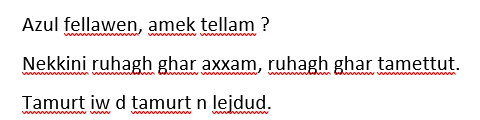
\includegraphics[width=0.96\linewidth]{images/vagues-rouges.png}}\\[0.3em]
  {\small\color{doux}Avant : Word souligne tout en rouge.}
\end{minipage}\hfill
\begin{minipage}[t]{0.47\linewidth}\centering
  \fcolorbox{filet}{white}{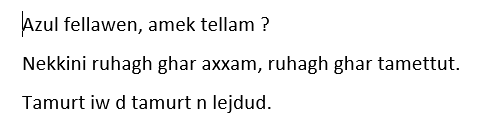
\includegraphics[width=0.96\linewidth]{images/sans-francais.png}}\\[0.3em]
  {\small\color{doux}Après « Ne pas vérifier en français ».}
\end{minipage}
\end{center}

\begin{enumerate}
  \item Sélectionnez le texte kabyle. \emph{S'il n'y a pas de sélection, c'est tout le document qui est concerné.}
  \item Cliquez sur \bouton{Ne pas vérifier en français}, dans l'onglet Kab-board. Le même lien existe en bas du volet.
\end{enumerate}
Ce réglage est enregistré avec le document. Le texte que vous tapez ensuite au même endroit en profite aussi. Pour un passage en français, sélectionnez-le et cliquez sur \bouton{Revérifier en français}.

% ---------------------------------------------------------------- 6
\section{Ouvrir le volet et attendre le correcteur}\label{s:volet}
Cliquez sur \bouton{Correcteur kabyle}. Le volet \textbf{Kab-board} s'ouvre à droite de la page :
\capture{volet-ouvert.png}{Le volet est prêt : « Correcteur prêt. Tout se calcule sur cet ordinateur. »}

\begin{encadre}{Le démarrage}
Le correcteur se prépare à chaque ouverture de Word : comptez \textbf{une quinzaine de secondes}, et jusqu'à une minute juste après avoir allumé l'ordinateur. Pendant ce temps, le volet affiche « Démarrage du correcteur… » et le bouton \bouton{Relire le document} reste grisé. Il s'active tout seul quand c'est prêt.
\end{encadre}
Le volet se ferme avec la croix en haut à droite, et se rouvre avec \bouton{Correcteur kabyle}.

% ---------------------------------------------------------------- 7
\section{Relire un document}\label{s:relire}
Cliquez sur \bouton{Relire le document}, dans le ruban ou dans le volet. Sur un long document, le volet montre la progression (« Relecture : paragraphe 12 sur 80… »), et \bouton{Annuler} l'arrête.
\capture{relecture.png}{Après la relecture : les mots douteux sont soulignés, et le volet montre le premier, avec ses propositions.}

Chaque mot douteux est souligné d'une vague de couleur :
\begin{itemize}
  \item \textcolor{vert}{\textbf{en vert}} quand le correcteur a tranché d'après la phrase : la première proposition est celle que le contexte désigne ;
  \item \textcolor{bleu}{\textbf{en bleu}} quand il propose seulement des formes proches du mot.
\end{itemize}
Le volet indique où vous en êtes (« Mot 1 sur 7 · 7 à revoir »), le mot en question, et jusqu'à six propositions. La première, en gras, est la meilleure.

\begin{encadre}[vert]{Rien n'est jamais remplacé sans vous}
Le correcteur ne fait que proposer. C'est toujours vous qui choisissez.
\end{encadre}

% ---------------------------------------------------------------- 8
\section{Corriger un mot}\label{s:corriger}
\subsection{Avec le clic droit (le plus rapide)}
Faites un \textbf{clic droit} sur un mot souligné. Ses propositions apparaissent en haut du menu habituel de Word. Cliquez sur la bonne :
\capture[0.6\linewidth]{menu-clic-droit.png}{Clic droit sur « tamettut » : les propositions, puis « Garder mon mot » et « Ajouter à mon dictionnaire ».}

\subsection{Avec le volet}
Cliquez sur un mot souligné dans le texte : le volet passe à ce mot, et votre curseur reste où vous avez cliqué. Choisissez une proposition dans la liste, puis :

\tableau{0.36\linewidth}{\textbf{Bouton} & \textbf{Effet}}{%
\bouton{Remplacer} & Remplace le mot par la proposition choisie, et passe au mot suivant. Un double-clic sur la proposition fait pareil. \\
\bouton{Remplacer partout} & Remplace toutes les fois où ce même mot est signalé (§\,\ref{s:partout}). \\
\bouton{Garder mon mot} & Vous aviez raison : le mot reste tel quel, ici. \\
\bouton{Ajouter à mon dictionnaire} & Le mot est juste et ne doit plus jamais être signalé, dans aucun document (§\,\ref{s:dictionnaire}). \\}

% ---------------------------------------------------------------- 9
\section{Remplacer partout}\label{s:partout}
Quand la même faute revient plusieurs fois, inutile de la corriger une à une. Choisissez la proposition, puis cliquez sur \bouton{Remplacer partout} :
\capture{remplacer-partout.png}{« ghar » remplacé par « ɣer » : 2 fois, d'un seul clic.}
Seules les occurrences encore à revoir de ce mot exact sont remplacées. Un seul \textbf{Ctrl+Z} les remet toutes.

% ---------------------------------------------------------------- 10
\section{Les possessifs : « tamurt iw » devient « tamurt-iw »}\label{s:possessifs}
Les possessifs s'attachent au nom par un trait d'union. Quand vous les écrivez séparés, le correcteur souligne \textbf{les deux mots ensemble} et propose la forme rattachée :
\capture{possessif.png}{« Tamurt iw » est signalé d'un bloc ; la proposition est « Tamurt-iw ».}
\bouton{Remplacer} remplace les deux mots d'un coup :
\capture[0.7\linewidth]{possessif-remplace.png}{Le résultat : « Tamurt-iw d tamurt n lejdud. »}
Le correcteur ne fusionne jamais deux mots séparés par une virgule.

% ---------------------------------------------------------------- 11
\section{Passer d'un mot à l'autre, arrêter la relecture}\label{s:naviguer}
\begin{minipage}[t]{0.38\linewidth}\vspace{0pt}\centering
  \fcolorbox{filet}{white}{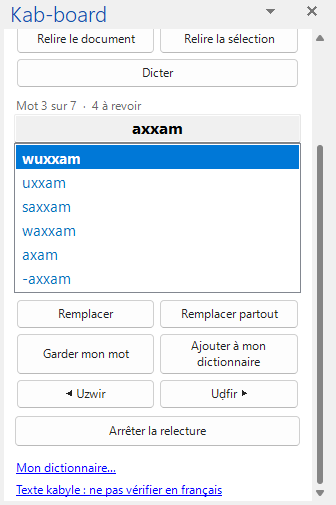
\includegraphics[width=0.94\linewidth]{images/volet-bas.png}}\\[0.3em]
  {\small\color{doux}Le bas du volet.}
\end{minipage}\hfill
\begin{minipage}[t]{0.58\linewidth}\vspace{0pt}
\begin{itemize}
  \item \bouton{$\blacktriangleleft$ Uzwir} : le mot précédent encore à revoir.
  \item \bouton{Uḍfir $\blacktriangleright$} : le mot suivant.
  \item Ou cliquez simplement sur un mot souligné dans le texte.
  \item \bouton{Arrêter la relecture} retire tous les soulignés de Kab-board.
  \item \textbf{Mon dictionnaire…} et \textbf{Texte kabyle : ne pas vérifier en français} : les mêmes que dans le ruban.
\end{itemize}
Sur un petit écran, faites défiler le volet pour voir ces boutons.
\end{minipage}

\medskip
Quand tout est revu, le volet l'indique : « Tout est revu ».

% ---------------------------------------------------------------- 12
\section{Relire seulement une partie}\label{s:partie}
Pour vérifier un passage sans relire tout le document :
\begin{enumerate}
  \item sélectionnez le passage, ou placez simplement le curseur dans un paragraphe ;
  \item cliquez sur \bouton{Relire la sélection}.
\end{enumerate}
Seuls ces paragraphes sont relus. Les soulignés déjà posés ailleurs restent en place. C'est pratique après avoir écrit ou dicté quelques phrases.

% ---------------------------------------------------------------- 13
\section{Mon dictionnaire}\label{s:dictionnaire}
Un nom propre, un mot régional, un mot juste que le correcteur ne connaît pas : ajoutez-le à \textbf{votre dictionnaire} et il ne sera plus jamais signalé.

\begin{minipage}[t]{0.4\linewidth}\vspace{0pt}\centering
  \fcolorbox{filet}{white}{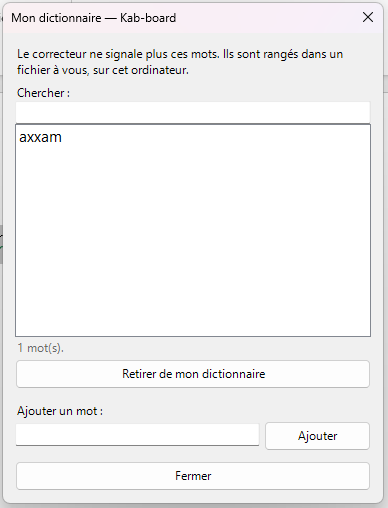
\includegraphics[width=0.94\linewidth]{images/dictionnaire.png}}\\[0.3em]
  {\small\color{doux}La fenêtre « Mon dictionnaire ».}
\end{minipage}\hfill
\begin{minipage}[t]{0.56\linewidth}\vspace{0pt}
\begin{itemize}
  \item Depuis un mot souligné : \bouton{Ajouter à mon dictionnaire} (volet ou clic droit).
  \item Pour voir et gérer la liste : \bouton{Mon dictionnaire} dans le ruban.
\end{itemize}
Dans cette fenêtre, vous pouvez :
\begin{itemize}
  \item \textbf{chercher} un mot dans la liste ;
  \item \textbf{retirer} un mot ajouté par erreur : sélectionnez-le, puis \bouton{Retirer de mon dictionnaire}, ou la touche Suppr ;
  \item \textbf{ajouter} un mot à la main : tapez-le en bas, puis \bouton{Ajouter}.
\end{itemize}
\end{minipage}

% ---------------------------------------------------------------- 14
\section{Dicter en kabyle}\label{s:dicter}
Kab-board peut écrire ce que vous dites, avec le même modèle de dictée que l'application sur téléphone.
\begin{enumerate}
  \item Placez le curseur là où le texte doit aller.
  \item Cliquez sur \bouton{Dicter}, dans le ruban ou dans le volet.
  \item Parlez normalement. Le bouton devient \bouton{Arrêter la dictée}.
  \item Cliquez sur \bouton{Arrêter la dictée} quand vous avez fini. Au bout de \textbf{30 secondes}, la dictée s'arrête toute seule.
\end{enumerate}
\capture{dictee.png}{Pendant l'écoute : « Arrêter la dictée » dans le ruban et dans le volet.}
Après quelques secondes de transcription, le texte s'écrit au curseur, dans votre graphie (v ou b). Il reste \textbf{sélectionné} : cliquez sur \bouton{Relire la sélection} pour le vérifier. La dictée n'est jamais corrigée d'office.

\begin{encadre}[ocre]{Si le micro ne marche pas}
Windows doit autoriser les applications de bureau à utiliser le micro : \emph{Paramètres\menu Confidentialité et sécurité\menu Microphone}, puis activez « Autoriser les applications de bureau à accéder à votre microphone ».
\end{encadre}
L'enregistrement de votre voix reste sur l'ordinateur et il est effacé dès que le texte est écrit.

% ---------------------------------------------------------------- 15
\section{Annuler, enregistrer, imprimer}\label{s:enregistrer}
\begin{itemize}
  \item \textbf{Annuler :} chaque correction, même un « Remplacer partout », s'annule d'un seul \textbf{Ctrl+Z}. Le mot rétabli redevient « à revoir ».
  \item \textbf{Enregistrer :} les soulignés de Kab-board ne vont \textbf{jamais} dans vos fichiers. Ils sont retirés juste avant l'enregistrement, puis remis. Un document envoyé par courriel ne les montre donc pas.
  \item \textbf{Imprimer :} même chose, les soulignés ne s'impriment pas.
  \item \textbf{Fermer :} si vous n'avez fait que relire, Word ne demande pas d'enregistrer pour les soulignés.
\end{itemize}
\begin{encadre}[ocre]{Enregistrement automatique (OneDrive)}
Avec l'enregistrement automatique de OneDrive, Word enregistre en continu, sans prévenir Kab-board. Cliquez sur \bouton{Arrêter la relecture} avant de partager un document.
\end{encadre}

% ---------------------------------------------------------------- 16
\section{Vos données}\label{s:donnees}
\textbf{Rien ne quitte votre ordinateur.} Le correcteur et la dictée tournent entièrement sur votre machine. Ils ne se connectent à aucun service sur Internet.

\tableau{0.3\linewidth}{\textbf{Quoi} & \textbf{Où}}{%
Le programme & \chemin{\%LOCALAPPDATA\%\bs Programs\bs Kab-board} \\
Votre dictionnaire & \chemin{\%LOCALAPPDATA\%\bs kab-board\bs mots-a-moi.txt} (un mot par ligne) \\
Le journal des incidents & \chemin{\%LOCALAPPDATA\%\bs kab-board\bs pont.log} \\
Votre graphie & dans le registre de Windows, à votre nom \\}

Pour ouvrir un de ces dossiers, tapez son chemin dans la barre d'adresse de l'Explorateur de fichiers.

% ---------------------------------------------------------------- 17
\section{Désinstaller}\label{s:desinstaller}
\begin{enumerate}
  \item Fermez Word.
  \item Ouvrez \emph{Paramètres\menu Applications\menu Applications installées}.
  \item Cherchez « Kab-board ».
  \item Cliquez sur les trois points \textbf{…} à droite de « Kab-board, correcteur kabyle pour Word », puis sur \bouton{Désinstaller}.
\end{enumerate}
\capture{desinstaller.png}{Kab-board dans la liste des applications installées.}
Votre dictionnaire est gardé, au cas où vous réinstalleriez. Pour l'effacer aussi, supprimez le dossier \chemin{\%LOCALAPPDATA\%\bs kab-board}.

% ---------------------------------------------------------------- 18
\section{En cas de souci}\label{s:souci}
\tableau{0.34\linewidth}{\textbf{Ce qui se passe} & \textbf{Que faire}}{%
L'onglet Kab-board n'apparaît pas & Fermez et rouvrez Word. Sinon : \emph{Fichier\menu Options\menu Compléments}, en bas « Gérer : Compléments COM »\menu\bouton{Atteindre}, et cochez « Kab-board ». Regardez aussi « Éléments désactivés » dans la même liste. \\ \addlinespace
« Relire » reste grisé & Le correcteur démarre encore : attendez que le volet affiche « Correcteur prêt ». Juste après avoir allumé l'ordinateur, cela peut prendre une minute. \\ \addlinespace
« Le correcteur s'est arrêté : il redémarre… » & Rien à faire : il repart tout seul. Si une relecture était en cours, elle reprend. \\ \addlinespace
« Le correcteur n'a pas pu démarrer » & Fermez Word et rouvrez-le. Si cela continue, réinstallez Kab-board. \\ \addlinespace
« Dicter » est grisé & Attendez « Correcteur prêt ». Le bouton est aussi grisé pendant une relecture. \\ \addlinespace
« Rien n'a été reconnu » & Parlez plus près du micro, et vérifiez l'autorisation du micro (§\,\ref{s:dicter}). \\ \addlinespace
Un mot juste est signalé & \bouton{Ajouter à mon dictionnaire}. \\}

Pour signaler un problème : \textbf{\href{https://github.com/ADJ-MSS/kab-board}{github.com/ADJ-MSS/kab-board}}. Joignez si possible le journal des incidents, \chemin{pont.log} (§\,\ref{s:donnees}).

Manuel en ligne, avec ceux du clavier pour Android et pour Linux :\newline \textbf{\href{https://kab-board-manuel-utilisation.netlify.app/word/}{kab-board-manuel-utilisation.netlify.app}}.

\end{document}
